\section{Results and Analysis}
\label{Results}

%Provide experiment results: serial \\
%Compare serial vs pthreads vs cuda vs theano. \\
%Provide graphs for speedup with increasing problem size \\
%Analyze speedup with number of threads/cores used \\
%Analyze the level of parallelization obtained \\
%Analyze performance bottlenecks \\
%Do overall analysis and compare obtained results with your expectations\\

As described in previous sections, we compare our implementations with state of the art deep learning library, Theano, in three different parallelizations (Serial/Pthreads/Cuda-C). All experiments are done under the same network structures with MNIST datasets and the number of threads is fixed as 32.

\begin{figure}[ht]
%\vskip 0.2in
\begin{center}
\centerline{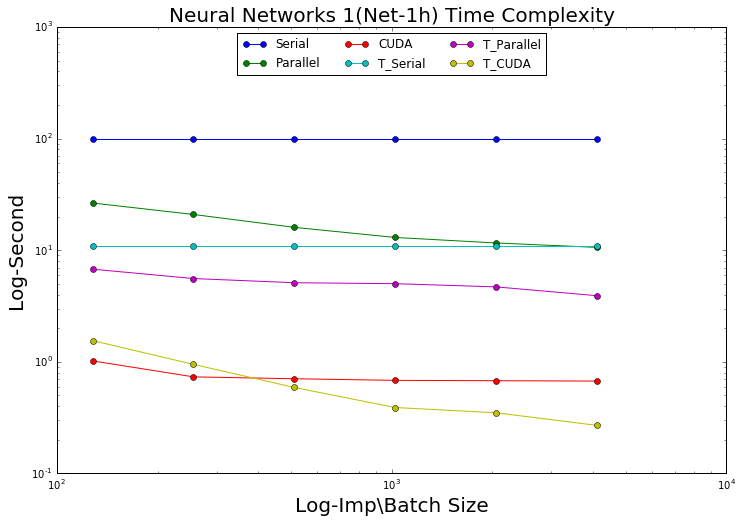
\includegraphics[width=\columnwidth]{../../slide/nn1_time.png}}
\caption{Learning time for Net-1h}
\label{fig:nn1_time}
\end{center}
\vskip -0.4in
\end{figure}

Figure \ref{fig:nn1_time} clearly shows distinct characteristics between serial and parallel computation as well as CPU and GPU based computation. First, the training time for 1 epoch of the serial implementation (Blue curve and Light blue curve) is almost constant over the varying mini batch size. It is obvious result because regardless of the size of each mini batch training data is accessed sequentially. On the other hand, the parallel learning time (Green curve) shows decreased training time due to multithreads distribution as we expected. One thing we should note is that the parallelism is enhanced when larger size of batch is used because the number of allocations of data into each thread is reduced. When smaller batch size is used, we need to assign each data into the corresponding thread more frequently and it causes more overheads. Moreover, as the last step, we need to combine all the results from every threads (which is called the reduction process) and the number of the reduction processes is also increased for smaller batch size. This behavior is shown commonly in the parallel computation based on Theano (T-Parallel).\\
In case of GPU based computation, the overall performance is significantly improved because GPU usually have much more cores which are specialized for repetitive operations such as matrix multiplications than CPU. As a result, GPU provides much faster learning time than that of CPU in general due to less number of allocation/reduction processes.\\
The faster computation by the parallelization is able to be captured by calculating GFLOPS. Figure \ref{fig:nn1_gflops} shows that parallelization provide much larger number of floating point operations than serial, thus, single thread computation.
\begin{figure}[ht]
%\vskip 0.2in
\begin{center}
\centerline{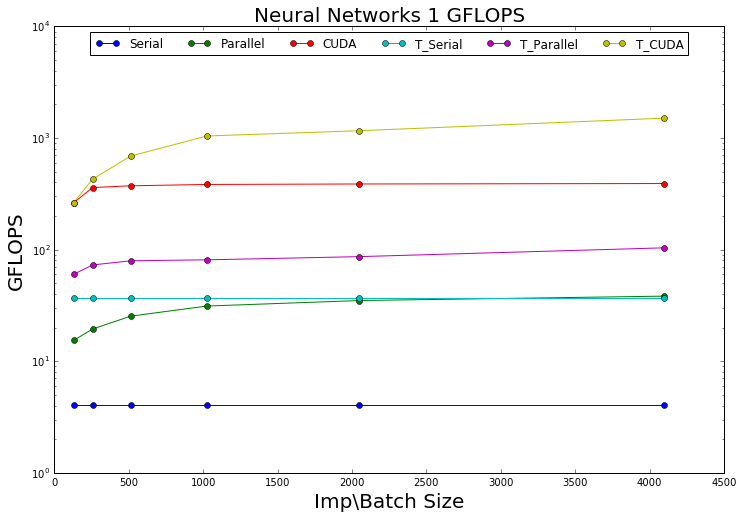
\includegraphics[width=\columnwidth]{../../slide/nn1_gflops.png}}
\caption{GFLOPS for Net-1h}
\label{fig:nn1_gflops}
\end{center}
\vskip -0.4in
\end{figure}

\textbf{BLAS} As Basic Linear Algebra Subprograms, BLAS has been crucial workhorse in heavy numerical computing. By replacing the self-built matrix-vector product libraries with BLAS functions, we could obtain hugely improved results (even faster than Theano). Note that the execution time of BLAS doesn't depend on the number of threads because it parallelizes each Matrix-vector product and hence each thread executes different parts of the same example. The serial implementation is still a bit slower than Theano but is faster than our previous implementation by about 10 times. This way shows that the optimized parallelism gives speed-up over Naive serial implementation. \\

\textbf{Bottleneck} In ideal case, by increasing the size of the batch, the number of overheads (allocation/reduction) is exponentially decreased. However, our experiment results show that there are some performance bottlenecks. In our implementation, shared memory bank conflicts which reduce the parallelism when threads access the shared memory appear when the number of batch increases. When the dimensions (i.e.number of neurons between layers) of the neural network is not perfect multiple of 32 then some threads do not participate in the computation so they are doing no work but still have to wait on the barrier. As a result, it causes degraded parallelism.\\

Overall, we demonstrate that the parallel computation is significantly faster than the serial computation by utilizing multithreads based on the mini batch in the multicore machine. Moreover, by dividing training datasets into larger mini batches, we are able to better performance than that of smaller batch size due to reduced overheads. Similarly, the training time and GFLOPS are improved in the second networks (Net-2h) (See Figure \ref{fig:nn2_time},\ref{fig:nn2_gflops}). 
\begin{figure}[ht]
%\vskip 0.2in
\begin{center}
\centerline{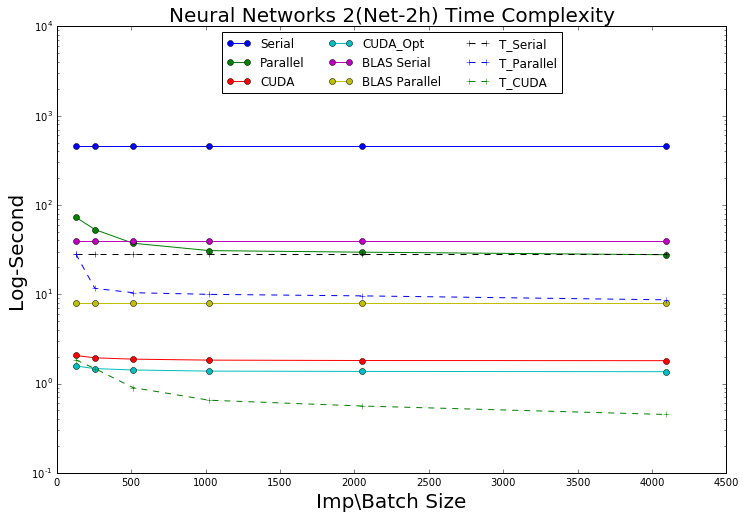
\includegraphics[width=\columnwidth]{../../slide/nn2_time.png}}
\caption{Learning time for Net-2h}
\label{fig:nn2_time}
\end{center}
\vskip -0.4in
\end{figure}
\begin{figure}[ht]
\vskip 0.2in
\begin{center}
\centerline{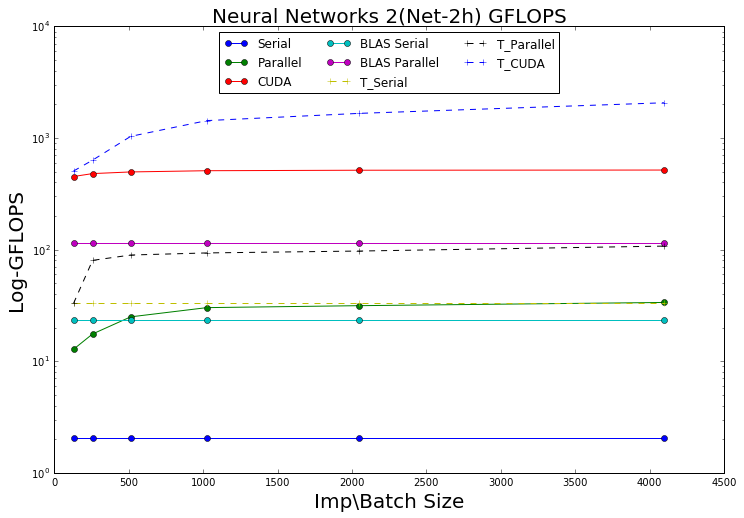
\includegraphics[width=\columnwidth]{../../slide/nn2_gflops.png}}
\caption{GFLOPS for Net-2h}
\label{fig:nn2_gflops}
\end{center}
\vskip -0.4in
\end{figure}



